\chapter{Mechanical Structure}

The mechanical structure is the physical backbone of the gantry system. Its two fundamental objectives are to bear the combined weight of the payload and the moving structure, and to provide smooth, low-friction linear motion along each axis. This chapter covers the trajectory-driven workspace requirements, the structural frame design, and the linear motion system selection.

\section{Trajectory-Driven Workspace Requirements}

Trajectory planning is presented in this chapter because the kinematic path of the end-effector directly determines the workspace envelope, clearance heights, and structural loads that govern the frame design. To validate these requirements, MATLAB was used to visualise the intended path of the end-effector in 3D space, confirming that the gantry can navigate from the home position, descend to grip the microwave, clear the box flaps, and place the object safely within.

The trajectory visualisation was developed under the following assumptions:
\begin{itemize}
    \item Static environment: the position of the pick-up zone and the packing box are fixed and known relative to the gantry's origin $(0, 0, 0)$.
    \item The expanded polystyrene (EPS) is estimated to be \SI{0.025}{m} in height; however, since this is soft, the height before placing the payload may differ from the height after impact.
    \item The end-effector and payload are treated as a concentrated point mass to focus on kinematic validity rather than complex dynamics.
    \item The motors can achieve the calculated quintic polynomial profiles for smooth curves and trapezoidal profiles for linear escape motions without saturation.
\end{itemize}

\begin{figure}[H]
    \centering
    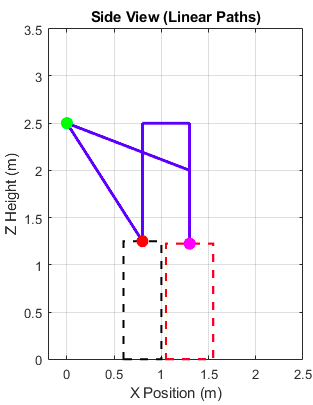
\includegraphics[width=0.75\linewidth]{figures/result_1.png}
    \caption{Side view of the linear trajectory segments showing pick, transfer, and place positions.}
    \label{fig:traj_side}
\end{figure}

\begin{figure}[H]
    \centering
    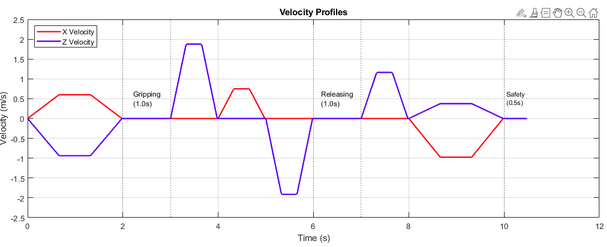
\includegraphics[width=1\linewidth]{figures/result_2.png}
    \caption{X and Z velocity profiles for the trajectory.}
    \label{fig:traj_vel}
\end{figure}

\begin{figure}[H]
    \centering
    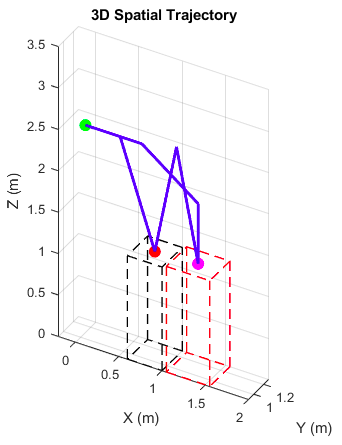
\includegraphics[width=0.75\linewidth]{figures/result_3.png}
    \caption{The 3D spatial trajectory of the end-effector through the pick-and-place cycle.}
    \label{fig:traj_3d}
\end{figure}

\begin{figure}[H]
    \centering
    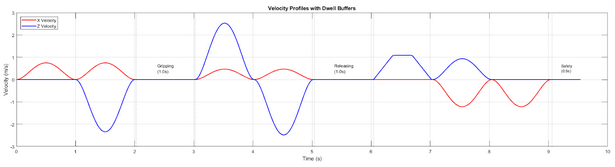
\includegraphics[width=1\linewidth]{figures/result_4.png}
    \caption{Velocity profiles with dwell buffers included for gripping and releasing operations.}
    \label{fig:traj_dwell}
\end{figure}

The trajectory reveals several key dependencies for the structural design. The vertical actuator stroke is directly dependent on a clearance height of \SI{2.6}{m}, required to navigate over the bin walls; the Z-axis mechanism must reach this apex from the pick point at \SI{1.25}{m}. The drop coordinate depends on the EPS padding thickness within the box, and must be adjustable to prevent impact damage. The structural frame height is set by the safety return height of \SI{2.0}{m}, ensuring the end-effector can clear all workspace obstacles.

The kinematic timing also has a direct relationship with dynamic loading: peak acceleration values are determined by segment durations, which in turn affect the required motor torque and belt tension. The initial control architecture decouples X and Z axis motion, which reduces cross-coupling errors and increases positional accuracy at the cost of longer cycle time. Simultaneous multi-axis motion (discussed in Section~9.3) can reduce cycle time but introduces greater dynamic loads.

\section{Frame Profile Selection}

Two structural profiles were evaluated for the main gantry frame: I-beams (Universal Beams) and C-section channels. Table~\ref{tab:frame_comparison} compares the two options.

\begin{table}[H]
    \centering
    \caption{Comparison of candidate frame profiles.}
    \label{tab:frame_comparison}
    \renewcommand{\arraystretch}{1.2}
    \begin{tabular}{@{}lcc@{}}
        \toprule
        \textbf{Criterion} & \textbf{I-Beam} & \textbf{C-Channel} \\
        \midrule
        Second moment of area & Higher (symmetric) & Lower (asymmetric) \\
        Bending resistance & Superior & Adequate \\
        Torsional rigidity & Moderate & Lower \\
        Cost (local market) & Higher & Lower \\
        Local availability & Good & Good \\
        Mounting complexity & Requires web drilling & Open flange simplifies mounting \\
        \bottomrule
    \end{tabular}
\end{table}

The I-beam was selected as the primary choice for its superior second moment of area and bending resistance, which are critical for supporting the moving carriage and payload across the \SI{4}{m} span without excessive deflection. The C-channel remains a viable cost-dependent alternative if budget constraints require it during final fabrication, as both profiles provide adequate structural safety margins for the design loads.

\section{Linear Motion System}

Two linear motion approaches were evaluated for guiding the carriages along the X and Y axes: castor wheels in aluminium extrusions, and recirculating linear guide blocks on hardened steel rails.

The castor wheel approach was tested on an early prototype. While inexpensive, the castor wheels exhibited excessive radial play and vibration under load, making them unsuitable for the positional accuracy required by the system. Recirculating linear guide blocks, which are standard in industrial gantry systems and were observed in use on existing machinery at the Dawlance plant (Figure~\ref{fig:plant_drive}), provide the required rigidity with negligible friction and were selected.

\begin{figure}[H]
    \centering
    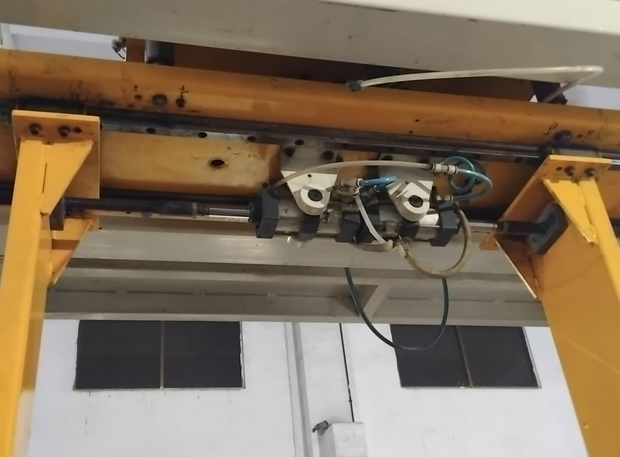
\includegraphics[width=0.75\linewidth]{figures/plant_driving.png}
    \caption{Linear guide rails on existing machinery at the Dawlance plant.}
    \label{fig:plant_drive}
\end{figure}

\subsection{Carriage Configuration}

The selected configuration uses four linear guide blocks per carriage, arranged in a rectangular ``car-like'' layout as shown in Figure~\ref{fig:4block}. A single- or double-block configuration was rejected because it would be susceptible to toppling under asymmetric loads. The four-block arrangement introduces a wide stance that effectively neutralises rolling and pitching moments. Furthermore, the Y-axis assembly is centred within the X-rails so that weight is distributed evenly and cantilever effects are eliminated.

\begin{figure}[H]
    \centering
    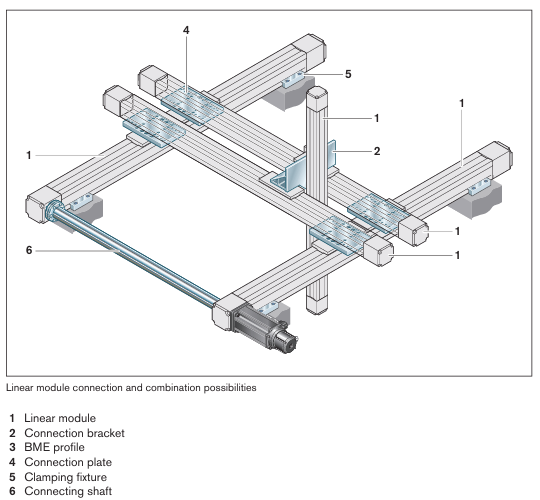
\includegraphics[width=0.75\linewidth]{figures/possibilities.png}
    \caption{Four-block carriage configuration for the primary axes~\cite{bosch_rexroth_linear}.}
    \label{fig:4block}
\end{figure}

\subsection{Service Life Estimation}

The linear guide service life was estimated using the $L_{10}$ methodology from the Bosch Rexroth and THK Linear Motion handbooks. The $L_{10}$ life represents the number of operating cycles (or equivalent distance) at which 90\% of a population of identical bearings would still be in service --- it is the standard reliability metric for rolling-element bearings.

A cumulative dynamic load of \SI{200}{kg} was defined as the worst case. This was derived from a \SI{40}{kg} payload multiplied by a dynamic application factor of 2.5 (yielding \SI{100}{kg}), added to a structural weight of \SI{55}{kg} and a safety margin of \SI{15}{kg}, giving \SI{170}{kg} static load rounded up to \SI{200}{kg} to account for peak dynamic forces. Table~\ref{tab:life_estimation} summarises the results.

\begin{table}[H]
    \centering
    \caption{Linear guide service life estimation under different loading scenarios.}
    \label{tab:life_estimation}
    \renewcommand{\arraystretch}{1.2}
    \begin{tabular}{@{}lcc@{}}
        \toprule
        \textbf{Configuration} & \textbf{Load per Block} & \textbf{Estimated $L_{10}$ Life} \\
        \midrule
        2-block, symmetric & 100\,kg & $\sim$24 years \\
        4-block, symmetric & 50\,kg & $\sim$12 years \\
        4-block, worst-case offset & 200\,kg (single block) & $\sim$8 years \\
        \bottomrule
    \end{tabular}
\end{table}

Even under worst-case offset loading where a single block bears the entire \SI{200}{kg}, the minimum service life of approximately 8 years exceeds the 10-year operational lifespan assumed in the economic analysis (Section~2.3.1), confirming durability.

\section{Design Parameter Summary}

Table~\ref{tab:design_parameters} summarises the locked design parameters for the mechanical structure. Drive system and motor parameters that were pending at the mechanical design stage have since been finalised and are detailed in Chapters~5 and~6.

\begin{table}[H]
    \centering
    \caption{Mechanical structure design parameters.}
    \label{tab:design_parameters}
    \small
    \renewcommand{\arraystretch}{1.2}
    \begin{tabularx}{\textwidth}{@{} p{2.1cm} p{2.4cm} p{2.2cm} X @{}}
        \toprule
        \textbf{Category} & \textbf{Parameter} & \textbf{Value} & \textbf{Notes} \\
        \midrule
        Load Capacity & Maximum dynamic load & 200\,kg & 40\,kg payload + structure + safety factor + $2.5\times$ dynamic multiplier. \\
        \addlinespace
        Workspace & Vertical escape height & 2.0\,m & Safety height to clear workspace obstacles (Figure~\ref{fig:traj_side}). \\
        \addlinespace
        Structure & Frame profile & I-Beam & Selected for bending resistance; C-channel as cost-dependent backup (Table~\ref{tab:frame_comparison}). \\
        \addlinespace
        Linear Motion & Bearing type & Linear guides & GHR-30 series; selected for precision and load capacity (Section~4.3). \\
        \addlinespace
        Linear Motion & Carriage config. & 4-block & Neutralises rolling/pitching moments (Figure~\ref{fig:4block}). \\
        \addlinespace
        Durability & $L_{10}$ life & $\geq 8$ years & Worst-case offset loading (Table~\ref{tab:life_estimation}). \\
        \addlinespace
        Drive System & X/Y actuator & HTD\,8M belt & Finalised in Chapter~5. \\
        \addlinespace
        Drive System & Z actuator & Rack \& pinion & Module~2, 20 teeth spur. Finalised in Chapter~5. \\
        \addlinespace
        Drive System & Motors & Yaskawa Sigma-5 & 400\,W (X, Y) and 200\,W (Z, yaw). Finalised in Chapter~6. \\
        \bottomrule
    \end{tabularx}
\end{table}

\section{Structural Prototype}

To evaluate the mechanical configurations and validate the axis designs prior to steel fabrication, a full-scale $4 \times 4 \times 2$\,m wooden frame was constructed. This frame served as the platform for testing linear guide installation, motor mounting, and drive mechanism integration. A detailed discussion of the prototype assembly and the testing performed on it is presented in Chapter~12.

\begin{figure}[H]
    \centering
    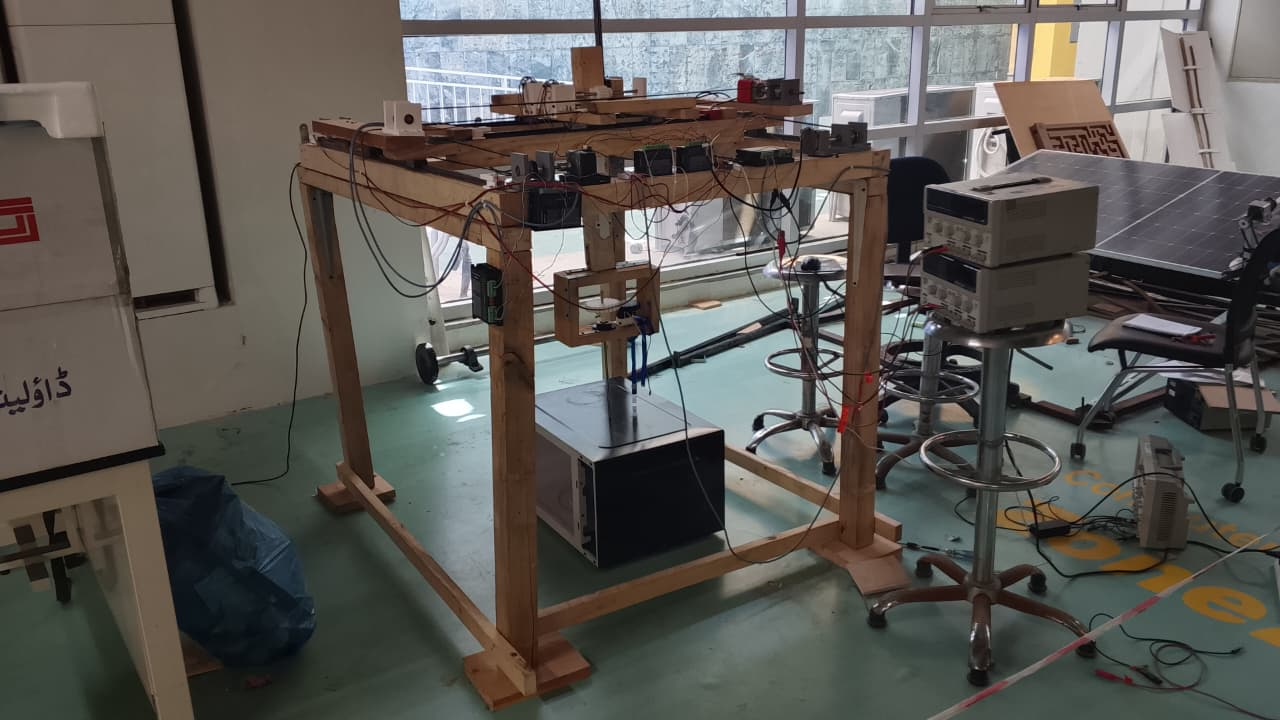
\includegraphics[width=\linewidth]{figures/gantry_image.jpeg}
    \caption{Wooden prototype with X-axis, Y-axis, Z-axis, and end-effector installed.}
    \label{fig:prototype_mech}
\end{figure}

The X-axis forms the primary load-bearing axis of the gantry, supporting the Y-axis carriage, Z-axis assembly, and end-effector. Two parallel X-bars act as the main rails, mechanically coupled using cross members to improve structural integrity and reduce deflection over the span. The Y-axis is mounted on the moving X-axis carriage, with linear guides installed perpendicular to the X-axis rails. The Y-bars are coupled to ensure rigidity while maintaining alignment with the X-axis structure, providing a stable moving platform for the Z-axis lifting mechanism.